\documentclass{beamer}
\usetheme{metropolis}
\usepackage{graphicx}
\usepackage{boolexpr}
\usepackage{kpfonts}
\usepackage{caption}
\usepackage{wrapfig}
\usepackage{tkz-graph}
\usepackage{tikz}
\usepackage{chngcntr}
\usepackage[labelformat=empty]{caption}
\usepackage[official]{eurosym}

\usepackage{siunitx}

\usepackage[math]{iwona}
\usepackage{scalerel}
\def\lVert{\mid\!\mid}
\def\rVert{\mid\!\mid}

\usepackage[normalem]{ulem}
\newcommand{\Adj}{\mathbf{A}}
\usepackage{mathtools}

\usepackage{custom}
\usepackage{amsfonts}
\newcommand{\jsrcodepath}{../../code}
\usepackage{jsr}

\newcommand{\expe}[2]{\la #1, #2 \ra}

\usepackage{framed}

\newcommand\Wider[2][3em]{%
\makebox[\linewidth][c]{%
  \begin{minipage}{\dimexpr\textwidth+#1\relax}
  \raggedright#2
  \end{minipage}%
  }%
}

\newcommand{\aeur}{\alpha_\text{\euro}}
\newcommand{\adol}{\alpha_\$}
\newcommand{\apou}{\alpha_\text{\pounds}}

\newcommand{\cssystemtikz}[2]{
  \begin{center}
    \begin{tikzpicture}[x=#1,y=#2]
      \Vertex{1}
      \NO[unit=4](1){2}
      \SOEA[unit=2](2){3}
      \EA[unit=2](3){4}
      \tikzset{EdgeStyle/.style = {->}}
      \tikzset{LoopStyle/.style = {->}}
      \tikzset{EdgeStyle/.append style = {bend right=18}}
      \Edge[label=1](1)(3)
      \Edge[label=3](1)(2)
      \Edge[label=2](2)(1)
      \Edge[label=1](2)(3)
      \Edge[label=2](3)(1)
      \Edge[label=3](3)(2)
      \Edge[label=4](3)(4)
      \draw[thick,->] (3) to [out=115,in=65,looseness=20] node [midway, fill=white] {1} (3);
      \Edge[label=1](4)(3)
    \end{tikzpicture}
  \end{center}
}

\title{Certifying unstability of Switched Systems using Sum of Squares Programming}
\date{}
\author{Beno\^it Legat (UCL), Rapha\"el M. Jungers (UCL) and Pablo A. Parrilo (MIT)}
\institute{Institute of Information and Communication Technologies, Electronics and Applied Mathematics (ICTEAM),\\
           Universit\'e catholique de Louvain (UCL)\\
           Laboratory for Information \& Decision Systems (LIDS)\\
           Massachusetts Institute of Technology (MIT)\\\\}

\begin{document}
  \maketitle
  \begin{frame}
    \tableofcontents
  \end{frame}
  \section{Introduction}
  \begin{frame}
      \frametitle{Motivation (from a Simulation viewpoint)}
      Analysis of integration method for $\dot{x} = Ax$ equivalent to analysis of dynamical systems\footnote{Based on joint work with Cl\'audio Gomes from the University of Antwerp}:
      \begin{center}
          \fbox{\parbox[m][9em][t]{0.33\textwidth}{
              Euler method:
              \begin{align*}
                  x_{k+1} &= x_k + h A x_k
              \end{align*}
              Midpoint method:
              \begin{align*}
                  x_{k+1} &= x_k + h A (x_k + \frac{h}{2}Ax_k)
              \end{align*}
          }}%
          $\Longleftrightarrow$%
          \fbox{\parbox[m][9em][t]{0.33\textwidth}{
              Euler method:
              \begin{align*}
                  e_{k+1} &= (I + hA)e_k + e_{\mathrm{local}}
              \end{align*}
              Midpoint method:
              \begin{align*}
                  e_{k+1} &= \Big(I + hA + \frac{h}{2}A^2\Big)e_k + e_{\mathrm{local}}
              \end{align*}
          }}
      \end{center}
      \uncover<2->{What happens if we \alert{switch} between the methods or step sizes ?}
      \uncover<3>{How can we compute the set of allowed switching sequences ?}
      \vspace{1em}
  \end{frame}

  \begin{frame}
      \frametitle{Example}
      Consider
      \begin{align*}
          A & =
          \begin{bmatrix}
              0 & 2\\
              0 & 0
          \end{bmatrix}&
          B & =
          \begin{bmatrix}
              0 & 0\\
              2 & 0
          \end{bmatrix}
      \end{align*}
      We have
      \begin{align*}
          \lim_{k \to \infty}& A \cdot A \cdot A \cdots = 0,&
          \lim_{k \to \infty}& B \cdot B \cdot B \cdots = 0,
      \end{align*}
      (in fact, $A$ and $B$ are nilpotent, so $A^2 = B^2 = 0$), but...
      \uncover<2->{
          \[ \lim_{k \to \infty} \norm{A \cdot B \cdot A \cdot B \cdots} = \infty \qquad \qquad (!) \]
      }
      \uncover<3>{
          The asymptotic growth rate of this sequence is 2, i.e.
          \[ \lim_{k \to \infty} \norm{(A \cdot B)^{\frac{k}{2}}}^{\frac{1}{k}} = 2 \]
      }
  \end{frame}

  \begin{frame}
      \frametitle{Joint spectral radius}
      Given a set of $n \times n$ matrices $\Sigma = \{A_1,\ldots,A_m\}$,
      what is the maximum ``growth rate'' that can be achieved by \alert{arbitrary switching}?
      \[ \rho(\Sigma) := \limsup_{k\to\infty} \max_{\sigma \in \{1,\ldots,m\}} \norm{A_{\sigma_k} \cdots A_{\sigma_2}A_{\sigma_1}}^{1/k}. \]

      Appeared in several different contexts: linear algebra (Rota-Strang 1960), wavelets (Daubechies-Lagarias 1992),
      switched linear systems, etc.

      \begin{itemize}
          \item If $m = 1$, ``standard'' spectral radius $\rho(A_1) = \max_i |\lambda_i|$.
          \item If $m \geq 2$, much more complicated...
      \end{itemize}
  \end{frame}

  \begin{frame}{Joint spectral radius is hard}
  Determining if $\rho(\Sigma) < 1$ is \alert{NP-hard} (Tsitsiklis \& Blondel 1997).

      \uncover<2->{Determining if $\rho(\Sigma) \leq 1$ is \alert{undecidable} (Blondel \& Tsitsiklis 2000).}


      \uncover<3->{
          Still, how to compute/approximate $\rho(\Sigma)$?

          What approximation guarantees can we have?

          How to produce ``bad'' switching sequences?
      }
  \end{frame}

  \begin{frame}{\only<2->{Constrained }Switched Systems}
    \begin{minipage}{0.23\textwidth}
      \[ x_{k+1} = A_{\sigma_k} x_k \]
      where \[A_{\sigma_k} \in \mathcal{M} \subseteq \R^{n \times n}.\]
    \end{minipage}
    \uncover<2->{%
      \begin{minipage}{0.75\textwidth}
        \cssystemtikz{50}{30}
      \end{minipage}
    }
    \begin{block}{\only<2->{Constrained }Joint Spectral Radius}
        \[ \only<1>{\jsr}\only<2>{\cjsr} = \lim_{k \to \infty} \max \norm{A_{\sigma_k} \cdots A_{\sigma_1}}^{1/k}.
      \]
      \uncover<2->{$\sigma_1, \ldots, \sigma_k$ is a path.}
    \end{block}
  \end{frame}


  \section{Lyapunov functions and their Sum of Squares Approximation}

  \begin{frame}
      \frametitle{Lyapunov function}
      \begin{block}{Theorem}
          Let $f(x)$ be a strictly positive homogeneous function,
          that satisfies
          \[ f(A_\sigma x) \leq \gamub f(x), \qquad \forall x \in \R^n, \sigma = 1, \ldots, m. \]
          Then $\jsr \leq \gamub$.
      \end{block}
  \end{frame}

  \begin{frame}
      \frametitle{Using SOS}
      We need a homogeneous polynomials $p(x)$ that satisfies
      \[ p(x) \geq 0, \qquad \gamub^{2d}p(x) - p(A_\sigma x) \geq 0 \quad \sigma = 1, \ldots, m. \]
      While this is not tractable, we can use instead
      \[ p(x) \text{ is SOS}, \qquad \gamub^{2d}p(x) - p(A_\sigma x) \text{ is SOS}\quad \sigma = 1, \ldots, m. \]
      Then $\jsr \leq \ujsrsos := \gamub$.

      For fixed $\gamub$, this is an SOS program, can be solved using an SDP solver.
  \end{frame}

  \begin{frame}{Example}
      Based on (Ando and Shih 98). Consider the two matrices:
      \[
          A_1 =
          \begin{bmatrix}
              1 & 0\\
              1 & 0
          \end{bmatrix},
          A_2 =
          \begin{bmatrix}
              0 & 1\\
              0 & -1
          \end{bmatrix},
      \]
      \begin{itemize}
          \item The true spectral radius is $\rho(A_1, A_2) = 1$.
          \item A common quadratic Lyapunov function (i.e. $d = 2$),
              gives $\rho(A_1, A_2) \leq \sqrt{2}$.
      \end{itemize}
  \end{frame}

  \begin{frame}{Example (cont.)}
      \begin{columns}
          \begin{column}{.6\textwidth}
              A quartic SOS Lyapunov function is enough to prove an upper bound
              of $1+\epsilon$ for \emph{every} $\epsilon > 0$, since
              \[ V(x) = (x_1^2 - x_2^2)^2 + \epsilon (x_1^2 + x_2^2)^2 \]
          \end{column}
          \begin{column}{.4\textwidth}
              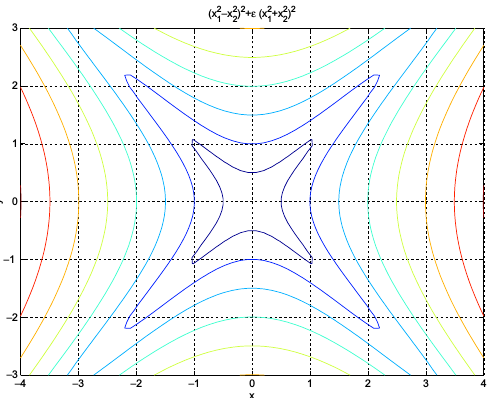
\includegraphics[trim=0cm 0cm 0cm .6cm, clip, width=\textwidth]{../../latex/images/polynomial.png}
          \end{column}
      \end{columns}
      satisfies
      \begin{align*}
          (1+\epsilon)V(x) - V(A_1x) &= (x_2^2-x_1^2 + \epsilon(x_1^2+x_2^2))^2\\
          (1+\epsilon)V(x) - V(A_2x) &= (x_1^2-x_2^2 + \epsilon(x_1^2+x_2^2))^2.
      \end{align*}

      \uncover<2>{What (if anything) can we say about approximation properties?}
  \end{frame}

  \begin{frame}
      \frametitle{SOS Guarantees}
      The degree-$d$ SOS upper bound for $\rho(A_1, \ldots,A_m)$ satisfies
      \[ \eta^{-\frac{1}{2d}} \ujsrsos \leq \jsr \leq \ujsrsos \]
      where $\eta = \min\Big\{m, {n+d-1 \choose d}\Big\}$.
      \begin{itemize}
          \item As degree $d \to \infty$, approx. ratio goes to 1!
      \end{itemize}
      \uncover<2>{
          But...
          \begin{itemize}
              \item How to generalize to \emph{constrained} switching?
              \item How to produce ``bad'' switching sequences?
          \end{itemize}
      }
      \vfill
      {\scriptsize
      P.A. Parrilo and A. Jadbabaie,
      Approximation of the joint spectral radius using sum of squares,
      \emph{Linear Algebra and its Applications},
      Vol. 428, No. 10, pp.~2385--2402, 2008.
      }
  \end{frame}

  \begin{frame}{Constrained Switching Systems and multi-Lyapunov}
      \null{}
      \vspace{-2.5em}
      \begin{center}
        \begin{tikzpicture}[x=50,y=20]
          \Vertex{1}
          \NO[unit=4](1){2}
          \SOEA[unit=2](2){3}
          \EA[unit=2](3){4}
          \tikzset{EdgeStyle/.style = {->}}
          \tikzset{LoopStyle/.style = {->}}
          \tikzset{EdgeStyle/.append style = {bend right=18}}
          \only<1-2>{
            \Edge[label=1](1)(3)
            \Edge[label=3](1)(2)
            \Edge[label=2](2)(1)
            \Edge[label=1](2)(3)
            \Edge[label=2](3)(1)
            \Edge[label=3](3)(2)
            \Edge[label=4](3)(4)
            \draw[thick,->] (3) to [out=115,in=65,looseness=20] node [midway, fill=white] {1} (3);
            \Edge[label=1](4)(3)
          }
        \end{tikzpicture}
      \end{center}
      \uncover<2->{
          \[ u \to_\sigma v \qquad f_v(A_{\sigma}x) \leq \gamub f_u(x). \]
          The degree-$d$ SOS upper bound satisfies
          \[ \eta^{-\frac{1}{2d}} \jsrsos \leq \cjsr \leq \jsrsos \]
          where $\eta = {n+d-1 \choose d}$.
      }

      \vfill

      {\scriptsize
      M. Philippe, R. Essick, G. Dullerud and R.M. Jungers, Stability of discrete-time switching systems with constrained switching sequences, \emph{arXiv preprint arXiv:1503.06984}, 2015}
  \end{frame}
  \begin{frame}{multi-Lyapunov functions}
    \Wider{
      \begin{center}
        \tabulinesep=0.5mm
        \begin{tabu}{{X[.7,c,m]X[c,m]X[c,m]X[c,m]X[c,m]}}
          & Node 1 & Node 2 & Node 3 & Node 4\\
          \PrimalFig{2}{1}
          \PrimalFig{4}{2}
          \PrimalFig{12}{6}
        \end{tabu}
      \end{center}
    }
  \end{frame}
  \begin{frame}{SOS Program}
    \begin{align*}
      \inf \gamub\\
      p_v(x) & \text{ is SOS} & \forall v \in \Nodes\\
      \gamub^{2d} p_u(x) - p_v(A_\sigma x) & \text{ is SOS} & \forall (u, v, \sigma) \in \Arcs.
    \end{align*}

      \uncover<2>{
          Last but not least...
          \begin{itemize}
              \item How to produce ``bad'' switching sequences?
          \end{itemize}
      }
  \end{frame}

  \section{Measures containing unstable trajectories and their moment relaxation}
  \begin{frame}{Drawing measures}
    A measure is \emph{atomic} if it is a sum of Diracs.

    Measures defined on
    \[
      \Sn = \{\, x : \|x\|_2 = 1\,\}
    \]
    so \alert{amplitude} in drawing represents
    \begin{itemize}
      \item \alert{mass} of atom for \emph{atomic measure},
      \item \alert{density} otherwise.
    \end{itemize}
    \begin{center}
      \begin{tikzpicture}
        \begin{scope}[shift={(-4,0)}]
          \draw[thick,->] (0,0) to (0,1);
          \fill (0,0) circle(.05);
          \node at (0,-.5) {$\delta_{(0, 1)}$};
        \end{scope}
        \begin{scope}[shift={(-2,0)}]
          \draw[thick,->] (0,0) to (0,2);
          \fill (0,0) circle(.05);
          \node at (0,-.5) {$2\delta_{(0, 1)}$};
        \end{scope}
        \begin{scope}[shift={(0,0)}]
          \draw[thick,->] (0,0) to (0.5,0);
          \fill (0,0) circle(.05);
          \node at (0,-.5) {$0.5\delta_{(1, 0)}$};
        \end{scope}
        \begin{scope}[shift={(3,0)}]
          \draw[thick,->] (0,0) to (0,2);
          \draw[thick,->] (0,0) to (0.5,0);
          \fill (0,0) circle(.05);
          \node at (0,-.5) {$2\delta_{(0, 1)} + 0.5\delta_{(1, 0)}$};
        \end{scope}
        \begin{scope}[shift={(6,0)}]
          \draw (0,0) circle(1);
          \fill (0,0) circle(.05);
          \node at (0,-.5) {Uniform};
        \end{scope}
      \end{tikzpicture}
    \end{center}
  \end{frame}

  \begin{frame}{Transfer/Frobenius-Perron operator and push-forward measure}
    Usual definition:
    \[ (\pushf{A}{\mu})(B) = \mu(A^{-1}(B)) \]
    \alert{Problem}: $\Sn$ not invariant under $A_\sigma$.

    \alert{Solution}: Alternative definition:
    \[ \int_{\Sn} f(x) (\pushf{A}{\mu})(\dif x) = \int_{\Sn} f(Ax) \mu(\dif x) \qquad \forall f. \]

    \begin{alert}{Example}
      $A = $ rotation by \ang{90} + 1.2 scaling
    \end{alert}

    \begin{center}
      \begin{tikzpicture}
        \begin{scope}[shift={(-3,0)}]
          \draw[thick,->] (0,0) to (0,2);
          \draw[thick,->] (0,0) to (0.5,0);
          \fill (0,0) circle(.05);
          \node at (0,-.5) {$\mu$};
        \end{scope}
        \begin{scope}[shift={(4,0)}]
          \draw[thick,->] (0,0) to (-2.4,0);
          \draw[thick,->] (0,0) to (0,0.6);
          \fill (0,0) circle(.05);
          \node at (0,-.5) {$\pushf{A}{\mu}$};
        \end{scope}
      \end{tikzpicture}
    \end{center}
  \end{frame}

  \begin{frame}{Periodic trajectory}
    Periodic trajectory of growth rate $\gamma$:
    \[ \gamma^k x_0 = A^k x_0 \]
    Let $x_i$, $1 \leq i \leq k$, be such that:
    \[ \gamma x_{i+1} = A x_i \]
    \begin{alert}{Example}
      \begin{center}
        \begin{tikzpicture}
          \begin{scope}[shift={(0,0)}]
            \draw[thick,->] (0,0) to (0.5,0);
            \node[above] at (0.5,0) {$x_1$};
            \fill (0,0) circle(.05);
            \node at (0,-1.5) {$k=1$};
          \end{scope}
          \begin{scope}[shift={(3,0)}]
            \draw[thick,->] (0,0) to (0,0.6);
            \node[right] at (0,0.6) {$x_2$};
            \fill (0,0) circle(.05);
            \node at (0,-1.5) {$k=2$};
          \end{scope}
          \begin{scope}[shift={(6,0)}]
            \draw[thick,->] (0,0) to (-0.72,0);
            \node[below] at (-0.72,0) {$x_3$};
            \fill (0,0) circle(.05);
            \node at (0,-1.5) {$k=3$};
          \end{scope}
          \begin{scope}[shift={(9,0)}]
            \draw[thick,->] (0,0) to (0,-0.864);
            \node[left] at (0,-0.864) {$x_4$};
            \fill (0,0) circle(.05);
            \node at (0,-1.5) {$k=4$};
          \end{scope}
        \end{tikzpicture}
      \end{center}
    \end{alert}
  \end{frame}

  \begin{frame}{Periodic trajectory as atomic measure I}
    Equivalent to:
    \[ \gamma \delta_{x_{k+1}} = \pushf{A}{\delta_{x_k}} \]
    \begin{alert}{Example}
      \begin{center}
        \begin{tikzpicture}
          \begin{scope}[shift={(0,0)}]
            \draw[thick,->] (0,0) to (0.5,0);
            \fill (0,0) circle(.05);
            \node at (0,-1.5) {$\delta_{(1,0)}$};
          \end{scope}
          \begin{scope}[shift={(3,0)}]
            \draw[thick,->] (0,0) to (0,0.6);
            \fill (0,0) circle(.05);
            \node at (0,-1.5) {$1.2\delta_{(0,1)}$};
          \end{scope}
          \begin{scope}[shift={(6,0)}]
            \draw[thick,->] (0,0) to (-0.72,0);
            \fill (0,0) circle(.05);
            \node at (0,-1.5) {$1.2^2\delta_{(-1,0)}$};
          \end{scope}
          \begin{scope}[shift={(9,0)}]
            \draw[thick,->] (0,0) to (0,-0.864);
            \fill (0,0) circle(.05);
            \node at (0,-1.5) {$1.2^3\delta_{(0,-1)}$};
          \end{scope}
        \end{tikzpicture}
      \end{center}
    \end{alert}
  \end{frame}

  \begin{frame}{Periodic trajectory as atomic measure II}
    Convexification: Find $\mu_{k}$ such that for all $k = 1, \ldots$
    \[ \gamma \mu_{k+1} = \pushf{A}{\mu_k}. \]
    Project the time:
    \[ \gamma \mu = \pushf{A}{\mu}. \]
    \begin{alert}{Example}
      \begin{center}
        \begin{tikzpicture}
          \begin{scope}[shift={(-3,0)}]
            \draw[thick,->] (0,0) to (0.5,0);
            \draw[thick,->] (0,0) to (0,0.6);
            \draw[thick,->] (0,0) to (-0.72,0);
            \draw[thick,->] (0,0) to (0,-0.864);
            \fill (0,0) circle(.05);
            \node at (0,-1.5) {$\mu$};
          \end{scope}
          \begin{scope}[shift={(3,0)}]
            \draw[thick,->] (0,0) to (0.6,0);
            \draw[thick,->] (0,0) to (0,0.72);
            \draw[thick,->] (0,0) to (-0.864,0);
            \draw[thick,->] (0,0) to (0,-1.0368);
            \fill (0,0) circle(.05);
            \node at (0,-1.5) {$\pushf{A}{\mu}$};
          \end{scope}
        \end{tikzpicture}
      \end{center}
    \end{alert}
  \end{frame}

  \begin{frame}{Measures containing unstable trajectories}
      \begin{block}{Theorem}
          Let $\mu_{\sigma}$, $\sigma=1, \ldots, m$, be measures on $\mathbb{S}^{n-1}$,
          that satisfies
          \[ \sum_{\sigma = 1}^m \pushf{A_\sigma}{\mu_\sigma} \geq \gamlb \sum_{\sigma = 1}^m \mu_\sigma, \]
          and at least one of the expectations is nonzero.

          Then  $\jsr \geq \gamlb$.
      \end{block}
  \end{frame}


  \begin{frame}{Conversion between periodic trajectory and atomic measures}
      Given a \emph{periodic} trajectory of growth rate $\gamma$,
      we can build \emph{atomic} measures for $\gamlb = \gamma$.

      Given \emph{atomic} measures for $\gamlb = \gamma$,
      we can build a \emph{periodic} trajectory of growth rate $\gamma$.

      \begin{block}{Example}
      Let
      \[ \A = \{ A_1 = e_1e_2^\Tr , A_2 = e_2e_1^\Tr  \} \]


      Measures with $\gamlb = 1$ are given by $\mu_1 = \delta_{(0,1)}$ and $\mu_2 = \delta_{(1,0)}$.

      \begin{center}
      \begin{tikzpicture}
          \begin{scope}[shift={(-7,0)}]
              \draw[thick,->,green] (0,0) to (0,1);
              \fill (0,0) circle(.05);
              \node at (0,-.5) {$\mu_1(x)$};
          \end{scope}

          \begin{scope}[shift={(-5,0)}]
              \draw[thick,->,blue] (0,0) to (1,0);
              \fill (0,0) circle(.05);
              \node at (0,-.5) {$\mu_2(x)$};
          \end{scope}

          \begin{scope}[shift={(-2,0)}]
              \draw[thick,->,green] (0,0) to (1,0);
              \draw[thick,->,blue] (0,0) to (0,1);
              \fill (0,0) circle(.05);
              \node at (0,-.5) {$\pushf{A_1}{\mu_1} + \pushf{A_2}{\mu_2}$};
          \end{scope}

          \begin{scope}[shift={(0,0)}]
              \node at (0,0) {$\geq$};
          \end{scope}

          \begin{scope}[shift={(2,0)}]
              \draw[thick,->,green] (0,0) to (0,1);
              \draw[thick,->,blue] (0,0) to (1,0);
              \fill (0,0) circle(.05);
              \node at (0,-.5) {$\mu_1(x) + \mu_2(x)$};
          \end{scope}
      \end{tikzpicture}
  \end{center}
      \end{block}
  \end{frame}


  \begin{frame}{Moment Program}
      Given the moments $\pmu$ up to degree $2d$,
      we can write the constraint
      \[
          \la \pmu, p(x) \ra = \int_{\mathbb{S}^{n-1}} p(x) \dif \pmu \geq 0, \qquad \forall p(x) \text{ SOS of degree }2d.
      \]
      as Semidefinite Programming constraints [Lasserre 2001].

      The moment relaxation of our program is:
      \begin{align}
          \notag
          \sup_{\pmu_{uv\sigma} \in \Soshd, \gamlb \in \R} \gamlb\\
          \notag
          \sum_{(u,v,\sigma) \in \Arcs} \pushf{A_\sigma}{\pmu_{uv\sigma}} & \succeq \gamlb^{2d} \sum_{(v,w,\sigma) \in \Arcs} \pmu_{vw\sigma}, \forall v \in \Nodes,\\
          \notag
          \sum_{(u,v,\sigma) \in \Arcs} \la \pmu_{uv\sigma}, \sum_{i=1}^n x_i^{2d} \ra & = 1.
      \end{align}
      This program is \emph{dual} to the sos program.
  \end{frame}

  \begin{frame}{When we have luck}
      If we find moments such that
      \[ \sum_{\sigma=1}^m \mathcal{A}_\sigma \pmu_\sigma - \gamlb^{2d} \sum_{\sigma = 1}^m \pmu_\sigma \]
      is a measure then $\gamlb \leq \jsr$.

      \begin{itemize}
          \item If this happens for $\gamlbopt$ then $\gamlbopt = \jsr = \gamubopt$
          \item In practice we can try to decompose the $\mu_\sigma$'s as a sum of diracs although it can only works if $\gamlb < \jsr$ or $\gamlb = \jsr$ and the system has the finiteness property.
      \end{itemize}
  \end{frame}

  \begin{frame}{Building a high growth sequence}
      \vspace{-1em}
    \Wider{\[ \sum_{(u,v,\sigma) \in E} \expe{\pmu_{uv\sigma}}{p(A_\sigma x)} \geq \gamlb^{2d}\sum_{(v,w,\sigma) \in \Arcs} \expe{\pmu_{vw\sigma}}{p(x)}, \qquad \forall v \in \Nodes, p(x) \text{ SOS}, \]
    \begin{center}
      \begin{tikzpicture}
        \SetGraphUnit{1.2}
        \GraphInit[vstyle=Dijkstra]
        \SetUpEdge[style={->}]
        \uncover<1,2>{\Vertex[L=$v$]{0}}
        \uncover<3->{\Vertex[L=$v_1$]{0}}
        \uncover<1,2,3>{\NOWE[L=$1$](0){4};}
        \uncover<4>{\NOWE[L=$v_2$](0){4};}
        \uncover<1-3>{\NOEA[L=$2$](0){5};}
        \uncover<1,2>{
          \SOWE[L=$3$](0){10};
          \SO[L=$4$](0){11};
          \SOEA[L=$5$](0){12};
        }
        \uncover<3->{
          \SOWE[L=$v_0$](0){10};
          \tikzset{VertexStyle/.append style = {dashed}}
          \SO[L=$4$](0){11};
          \SOEA[L=$5$](0){12};
        }
        \uncover<4>{\NOEA[L=$2$](0){5};}
        \uncover<1-3>{\Edge[label=$1$](4)(0);}
        \uncover<4>{\Edge[label=$\sigma_1$](4)(0);}
        \uncover<1-3>{\Edge[label=$2$](5)(0);}
        \uncover<1,2>{
          \Edge[label=$3$](0)(10);
          \Edge[label=$4$](0)(11);
          \Edge[label=$5$](0)(12);
        }
        \uncover<3->{
          \tikzset{EdgeStyle/.append style = {dashed}}
          \Edge[label=$\sigma_0$](0)(10);
          \Edge(0)(11);
          \Edge(0)(12);
        }
        \uncover<4>{\Edge[label=$2$](5)(0);}
      \end{tikzpicture}
    \end{center}
      Construct sequence \emph{backwards}, using ``best expectation'':
    \begin{align*}
      \uncover<2->{\expe{\pmu_{1v1}}{p(A_1 x)} + \expe{\pmu_{2v2}}{p(A_2 x)} & \geq \gamlb^{2d}(\expe{\pmu_{v33}}{p(x)} + \expe{\pmu_{v44}}{p(x)} + \expe{\pmu_{v55}}{p(x)}),\\}
      \uncover<3->{\expe{\pmu_{1v_11}}{p(A_1 x)} + \expe{\pmu_{2v_12}}{p(A_2 x)} & \geq \gamlb^{2d}\expe{\pmu_{v_1v_0\sigma_0}}{p(x)},\\}
      \uncover<4>{\expe{\pmu_{v_2v_1\sigma_1}}{p(A_1 x)} & \geq \frac{1}{2} \gamlb^{2d}\expe{\pmu_{v_1v_0\sigma_0}}{p(x)}.}
    \end{align*}
  }
  \end{frame}
  \begin{frame}[allowframebreaks]
    \frametitle{Algorithm for building a high-growth sequence}
    \begin{algorithmic}
      \STATE{Pick an arbitrary polynomial $p_0(x) \in \inte(\Sosh)$}
      \STATE{Pick an \arc{} $(v_1,v_0,\sigma_0) \in \Arcs$ such that $\la \mu_{v_1v_0\sigma_0}, p_0(x) \ra > 0$}
      \STATE{Set $p_1(x) \leftarrow p_0(x)$}
      \FOR{$k = 1,2,\ldots$}
      \STATE $(v_{k+1},v_k,\sigma_k) \leftarrow \argmax_{(u,v_k,\sigma) \in \Arcs} \la \mu_{uv_k\sigma}, p_k(A_\sigma x) \ra$
      \STATE $p_{k+1} \leftarrow p_k(A_{\sigma_k} x)$
      \ENDFOR
    \end{algorithmic}

    \begin{center}
      \begin{tikzpicture}
        \SetGraphUnit{2}
        \GraphInit[vstyle=Dijkstra]
        \SetUpEdge[style={->}]
        \Vertex[L=$p_0(x)$]{0}
        \NOWE[L=$p_0(A_{\sigma_1} x)$](0){4};
        \SOWE[L=$p_0(x)$](0){10};
        \tikzset{VertexStyle/.append style = {dashed}}
        \SO[L=$4$](0){11};
        \SOEA[L=$5$](0){12};
        \NOEA[L=$2$](0){5};
        \Edge[label=$\sigma_1$](4)(0);
        \tikzset{EdgeStyle/.append style = {dashed}}
        \Edge[label=$\sigma_0$](0)(10);
        \Edge(0)(11);
        \Edge(0)(12);
        \Edge[label=$2$](5)(0);
      \end{tikzpicture}
    \end{center}
  \end{frame}

  \begin{frame}{Let's try it}
    \begin{center}
      \begin{tikzpicture}[x=70,y=28]
        \Vertex{1}
        \NO[unit=4](1){2}
        \SOEA[unit=2](2){3}
        \EA[unit=2](3){4}
        \tikzset{EdgeStyle/.style = {->}}
        \tikzset{LoopStyle/.style = {->}}
        \tikzset{EdgeStyle/.append style = {bend right=18}}
        \Edge[label=1](1)(3)
        \Edge[label=2](3)(1)
        \draw[thick,->] (3) to [out=115,in=65,looseness=20] node [midway, fill=white] {1} (3);
        \uncover<2>{
          \Edge[label=3](1)(2)
          \Edge[label=1](2)(3)
        }
        \uncover<1>{
          \tikzset{EdgeStyle/.append style = {dashed}}
          \Edge[label=3](1)(2)
          \Edge[label=1](2)(3)
        }
        \tikzset{EdgeStyle/.append style = {dashed}}
        \Edge[label=2](2)(1)
        \Edge[label=3](3)(2)
        \Edge[label=4](3)(4)
        \Edge[label=1](4)(3)
      \end{tikzpicture}
      \hspace{1cm}
      \only<1>{
        $2d = 2$
        \[ 3 \to_2 1 \to_1 3 \to_2 1 \to_3 1 \to_1 3 \to_1 3 \to_1 3 \to_1 3 \to_1 3 \]
        $0.97\textcolor{red}{289}$
      }
      \only<2>{
        $2d = 12$
        \[ 3 \to_2 1 \to_1 3 \to_2 1 \to_3 2 \to_1 3 \to_1 3 \to_1 3 \to_1 3 \]
        $0.97\textcolor{green}{482}$
      }
    \end{center}
  \end{frame}
  \begin{frame}{Improvement}
    \only<1>{
      \begin{center}
      \begin{tikzpicture}
        \SetGraphUnit{1.2}
        \GraphInit[vstyle=Dijkstra]
        \SetVertexNoLabel
        \SetUpEdge[style={->}]
        \Vertex[NoLabel=false,L=$v_1$]{0}
        \NOWE(0){4};
        \NOEA(0){5};
        \SO[NoLabel=false,L=$v_0$](0){11};
        \tikzset{VertexStyle/.append style = {dashed}}
        \SOWE(0){10};
        \SOEA(0){12};
        \Edge[label=?](4)(0);
        \Edge[label=?](5)(0);
        \Edge(0)(11);
        \tikzset{EdgeStyle/.append style = {dashed}}
        \Edge(0)(10);
        \Edge(0)(12);
      \end{tikzpicture}
      \end{center}
    }
    \only<2>{
      \begin{center}
      \begin{tikzpicture}
        \SetGraphUnit{1.2}
        \GraphInit[vstyle=Dijkstra]
        \SetVertexNoLabel
        \SetUpEdge[style={->}]
        \Vertex[NoLabel=false,L=$v_1$]{0}
        \NOWE(0){4};
        \NOEA(0){5};
        \NOWE(4){6};
        \NO  (4){7};
        \NOEA(4){8};
        \NOEA(5){9};
        \SO[NoLabel=false,L=$v_0$](0){11};
        \tikzset{VertexStyle/.append style = {dashed}}
        \SOWE(4){1};
        \EA(0){2};
        \EA(2){3};
        \SOWE(0){10};
        \SOEA(0){12};
        \Edge[label=?](6)(4);
        \Edge[label=?](7)(4);
        \Edge[label=?](8)(4);
        \Edge[label=?](8)(5);
        \Edge[label=?](9)(5);
        \Edge[label=?](4)(0);
        \Edge[label=?](5)(0);
        \Edge(0)(11);
        \tikzset{EdgeStyle/.append style = {dashed}}
        \Edge(4)(1);
        \Edge(5)(2);
        \Edge(5)(3);
        \Edge(0)(10);
        \Edge(0)(12);
      \end{tikzpicture}
      \end{center}
    }
  \end{frame}
  \begin{frame}{Improved guarantee}
      With horizon 1:
      \[ \frac{\gamlb}{\norm{\Adj^\Tr}_\infty^{\frac{1}{2d}}} \leq \lim_{k \to \infty} \norm{A_{\sigma_1} \cdots A_{\sigma_k}}^{\frac{1}{k}}. \]

    With horizon $l$:
    \[ \frac{\gamlb}{\norm{[\Adj^\Tr]^l}_\infty^{\frac{1}{2dl}}} \leq \lim_{k \to \infty} \norm{A_{\sigma_1} \cdots A_{\sigma_k}}^{\frac{1}{k}}. \]
  \end{frame}
  \begin{frame}{Let's try it}
    \begin{center}
      \begin{tikzpicture}[x=70,y=28]
        \Vertex{1}
        \NO[unit=4](1){2}
        \SOEA[unit=2](2){3}
        \EA[unit=2](3){4}
        \tikzset{EdgeStyle/.style = {->}}
        \tikzset{LoopStyle/.style = {->}}
        \tikzset{EdgeStyle/.append style = {bend right=18}}
        \Edge[label=1](1)(3)
        \Edge[label=2](3)(1)
        \draw[thick,->] (3) to [out=115,in=65,looseness=20] node [midway, fill=white] {1} (3);
        \Edge[label=3](1)(2)
        \Edge[label=1](2)(3)
        \tikzset{EdgeStyle/.append style = {dashed}}
        \Edge[label=2](2)(1)
        \Edge[label=3](3)(2)
        \Edge[label=4](3)(4)
        \Edge[label=1](4)(3)
      \end{tikzpicture}
      \hspace{1cm}
      $2d = 2, l = 3$
      \[ 3 \to_2 1 \to_1 3 \to_2 1 \to_3 2 \to_1 3 \to_1 3 \to_1 3 \to_1 3 \]
      $0.97\textcolor{green}{482}$
    \end{center}
  \end{frame}

  \begin{frame}{Guarantee for the upper bound}
      \Wider{This yields, as $l \to \infty$,
      \[ \rho(\Adj)^{-\frac{1}{2d}}\jsrsos \leq \lim_{k \to \infty} \norm{A_{\sigma_1} \cdots A_{\sigma_k}}^{\frac{1}{k}} \leq \cjsr \leq \jsrsos. \]

      Practical improvements for lower bound:
      \begin{itemize}
          \item Use $\Adj(G')$ where edges of 0 dual variable are removed.
          \item Find lower bound in an high growth rate sequence produced.
      \end{itemize}}

      \vfill

      {\scriptsize
      B. L., R.M. Jungers and P.A. Parrilo,
      Generating unstable trajectories for Switched Systems via Dual Sum-Of-Squares techniques,
      \emph{Proceedings of the 19th International Conference on Hybrid Systems: Computation and Control},
      ACM, pp.~51--60, 2016.
      }
  \end{frame}
  \begin{frame}{Implementation}
      \begin{center}
        \begin{tikzpicture}[x=26,y=45]
          \SetVertexNormal[Shape=rectangle,FillColor = red!50]
          \Vertex[x=0,y=0,L={\jlpkg{SwitchOnSafety}}]{SS}
          \SetVertexNormal[Shape=rectangle,FillColor = blue!30]
          \Vertex[x=0,y=-1,L={\jlpkg{PolyJuMP}}]{PJMP}
          \Vertex[x=4,y=-2,L={\jlpkg{JuMP}}]{JMP}
          \Vertex[x=0,y=-2.5,L={\jlpkg{SumOfSquares}}]{SOS}
          \SetVertexNormal[Shape=rectangle,FillColor = green!50]
          \Vertex[x=-3,y=-3,L={\jlpkg{MultivariatePolynomials}}]{MP}
          \Vertex[x=3,y=-3,L={\jlpkg{MathOptInterface}}]{MOI}
          \SetVertexNormal[Shape=rectangle,FillColor = yellow!50]
          \Vertex[x=-3,y=-4,L={\jlpkg{Mosek}}]{Mosek}
          \Vertex[x=-1,y=-4,L={\jlpkg{SCS}}]{SCS}
          \Vertex[x=1,y=-4,L={\jlpkg{CSDP}}]{CSDP}
          \Vertex[x=3,y=-4,L={\jlpkg{SDPA}}]{SDPA}
          \tikzset{EdgeStyle/.style={->}}
          \Edge(SS)(PJMP)
          \Edge(PJMP)(MP)
          \Edge(PJMP)(SOS)
          \Edge(PJMP)(JMP)
          \Edge(JMP)(MOI)
          \Edge(MOI)(Mosek)
          \Edge(MOI)(SCS)
          \Edge(MOI)(CSDP)
          \Edge(MOI)(SDPA)
        \end{tikzpicture}
      \end{center}
  \end{frame}
  \section{Conclusion}
  \begin{frame}{Conclusion}
    \begin{block}{Results}
      \begin{itemize}
        \item Approximation guarantees depending on $d$ and $\rho(\Adj)$.
        \item New algorithm for producing high-growth sequences.
        \item New lower bound certificates using measures.
        \item Convex program provides both upper and lower bounds.
      \end{itemize}
    \end{block}
    \begin{block}{Open questions}
      \begin{itemize}
        \item Improved guarantees? What is best possible?
        \item Is the sequence always periodic for a fixed $d$ ? Can we bound the period ?
      \end{itemize}
    \end{block}
  \end{frame}

  \begin{frame}{Why is it a relaxation ?}
  \Wider{
      The Semidefinite Programming constraints on the trunctated moments of $\mu_\sigma$ are necessary for the existence of a measure with those moments,
  and \alert{any} value of the moments of higher degree (not necessarily 0).

  In the Common Quadratic Lyapunov Function case, i.e. $2d = 2$, those conditions are necessary and sufficient.
  \begin{itemize}
      \item For every truncated moments, we can find a $\mu_\sigma$ that has these moments.
      \item And there exists a slack variable $\mu_{\mathrm{slack}}$ such that
          \[ \sum_{\sigma=1}^m \Exp_{\mu_\sigma}[p(A_\sigma x)] - \gamlb^{2d} \sum_{\sigma = 1}^m \Exp_{\mu_\sigma}[p(x)] = \Exp_{\mu_{\mathrm{slack}}}, \forall p(x) \in \Sosh, \]
          so
          \[ \sum_{\sigma=1}^m \mathcal{A}_\sigma \mu_\sigma - \gamlb^{2d} \sum_{\sigma = 1}^m \mu_\sigma \only<1>{=}\only<2>{\text{ has the same trunctated moments than }} \mu_{\mathrm{slack}} \]
  \end{itemize}
  }
\end{frame}

  \begin{frame}{Adjacency matrix}
  \Wider{\cssystemtikz{40}{20}%
    \uncover<2->{\[ \rho(\Adj) = \lim_{k \to \infty} \norm{\Adj^k}^{1/k}. \]}%
  \begin{minipage}{0.35\textwidth}
    \begin{align*}
      \only<1-3>{
        \Adj & =
        \begin{pmatrix}
          0 & 1 & 1 & 0\\
          1 & 0 & 1 & 0\\
          1 & 1 & 1 & 1\\
          0 & 0 & 1 & 0
        \end{pmatrix}.
      }
      \only<4>{
        \Adj^2 & =
        \begin{pmatrix}
          2 & 1 & 2 & 1\\
          1 & 2 & 2 & 1\\
          2 & 2 & 4 & 1\\
          1 & 1 & 1 & 1
        \end{pmatrix}.
      }
      \only<5>{
        \Adj^3 & =
        \begin{pmatrix}
          3 & 4 & 6 & 2\\
          4 & 3 & 6 & 2\\
          6 & 6 & 9 & 4\\
          2 & 2 & 4 & 1
        \end{pmatrix}.
      }
    \end{align*}
  \end{minipage}
  \begin{minipage}{0.6\textwidth}
    \begin{align*}
      \only<3>{
        \norm{\Adj}_\infty & = \max
        \begin{pmatrix}
          0 + 1 + 1 + 0\\
          1 + 0 + 1 + 0\\
          1 + 1 + 1 + 1\\
          0 + 0 + 1 + 0
        \end{pmatrix} =
        \begin{pmatrix}
          2\\2\\4\\1
        \end{pmatrix}.%
      }
      \only<4>{
        \norm{\Adj^2}_\infty & = \max
        \begin{pmatrix}
          2 + 1 + 2 + 1\\
          1 + 2 + 2 + 1\\
          2 + 2 + 4 + 1\\
          1 + 1 + 1 + 1
        \end{pmatrix} =
        \begin{pmatrix}
          6\\6\\9\\4
        \end{pmatrix}.%
      }
      \only<5>{
        \norm{\Adj^3}_\infty & = \max
        \begin{pmatrix}
          3 + 4 + 6 + 2\\
          4 + 3 + 6 + 2\\
          6 + 6 + 9 + 4\\
          2 + 2 + 4 + 1
        \end{pmatrix} =
        \begin{pmatrix}
          15\\15\\25\\9
        \end{pmatrix}.
      }
    \end{align*}
\end{minipage}}
\end{frame}

\end{document}
